\chapter{Probability over time}

When we discussed the theory of preferences in chapter~\ref{c:certainty}, we pointed out that the theory is {\it synchronic}; it's only about consistency at a given time.  One needs to obey the axioms today. One also needs to obey them tomorrow (and the next day, and the next).  But the axioms don't tell you how today relates to tomorrow. It doesn't tell you anything about preference change.  It doesn't violate the axioms that I switched my preference between candy and salad sometime in the last 40 years.

So far, the subjectivist theory of probability is the same.  It tells you how today-beliefs ought to cohere with other today-beliefs. It tells you how tomorrow-beliefs ought to cohere with other tomorrow-beliefs. What we have not yet discussed is how today-beliefs need to cohere with tomorrow-beliefs.

That might seem very strange thing to say, and you might find it perplexing.  So let's start with an example of what I mean.

Suppose that today Mandy's subjective probability in the event ``we'll find life on Mars'' is 0.6.  Suppose that Mandy dutifully obeys the probability axioms in all her beliefs, so she not subject to a book or distance argument.

Today Mandy forms a plan: When she wakes up tomorrow, her new probability for finding life on Mars is going to be 0.2. She doesn't think she's going to learn anything that is relevant to the question of life on Mars. She just wants to ``keep people on their toes.'' She plans to adjust all her other beliefs tomorrow to ensure that she is consistent with the probability axioms accordingly. She doesn't want to be irrational, after all.

Has Mandy done anything wrong? Is her plan rational?  If she follows through, would we think that was okay?  It sure seems weird.  Rationality, one might argue, should require you to only change your beliefs in response to learning something relevant.  Mandy is obeying the axioms, but is violating this other intuitive constraint.

\section{Conditional probability and Bayes theorem}

We didn't introduce it in the last chapter,  there is a type of probability called ``conditional probability.''  Often it is denoted with the symbol: $|$.  So, you would read: $P(F | E)$ as ``the probability of event $F$ conditional on $E$.'' In probability textbooks it is defined this way:
\begin{equation}
    \label{e:conditional-prob}
    P(F | E) = \frac{P(F \cap E)}{P(E)}
\end{equation}

\nomenclature{$|$}{Conditional probability. $P(E|F)$ is read as ``the probability of $E$ conditional on $F$.''}
\nomenclature{$\cap$}{Set theoretic intersection. $X \cap Y$ is the set which contains elements that are in both $X$ and $Y$ and no others.}

While conditional probability can mean many things, one common way of interpreting it is that it is the probability of $F$ after learning that $E$ happened.  This definition of conditional probability gives rise to the most famous equation in probability: {\it Bayes Theorem}. 

To understand Bayes' theorem, let's start with a simple example.  Suppose that Frick Honeydew University is developing their academic integrity policy.  FHU thinks that there are two basic types of students, those who are irredeemable cheaters and those who are not. It wants to know: when we catch a student cheating, how likely is it that this student is an irredeemable cheater versus a student who just made a stupid mistake?  It conducts a study of its students and faculty and estimates the following probabilities.

\marginnote{{\bf Please note}: these numbers are completely made up for the purposes of this example. They don't represent any real data about anything.} Most students are not irredeemable cheaters (event $I$), so the $P(I) = 0.05$. The probability that a an irredeemable cheater is caught cheating one time in their career (event $C$) is high, $P(C|I) = 0.8$. Good students make mistakes and cheat, even though they aren't irredeemable.  So, $P(C|\neg I) = 0.1$

\nomenclature{$\neg$}{Negation or set theoretic inverse. $\neg E$ means all the events in $\Omega$ which are not in $E$.}

Now FHU wants to know, when we catch a student cheating for the first time, what is the probability that they are an irredeemable cheater?  Notice we don't yet have that information. We know that {\it if} the student is irredeemable, then the probability that they will be caught is 0.9.  But what FHU wants to know is different. FHU wants to know {\it if} the student is caught, what the probability that they are irredeemable?

If you are struggling a bit with the difference between these two, consider this analogy.  Suppose that I choose a person currently living on Earth at random.  I know who they are, but you don't.  I decide to convey a little information to you: They live in the US.  What is the probability that they speak English?\marginnote{These numbers about English speakers are not made up by me, they come from Wikipedia.} As of 2022, it was about 90\%. It's not surprising that the vast majority of people who live in the US speak English. 

Now, suppose that I choose another person who llives on Earth at random. I tell you: They speak English.  What is the chance they live in the US? Now the number is much lower.  Why is it lower? There are many reasons.  First, English is the main language of several other countries (like the UK). Also, many countries have significant English-speaking populations (like India). And finally, English is becoming a very common second language for the global population.  The chance that a random English-speaking person lives in the US is more like 20\%. 

This shows the difference between the two conditional probabilities. The probability of speaking English conditional on living in the US and the probability of living in the US conditional on speaking English.

Now, we return to our example of Frick Honeydew University. FHU knows one direction: the probability that someone gets caught cheating conditional on being irredeemably a cheater (and not being that).  They want to know the opposite: the probability of being irredeemably a cheater given that they were caught cheating.  What should they do?  This is where Bayes' theorem comes in.

First let's list what we know:
\begin{align*}
    P(I) & = 0.05\\
    P(\neg I) &= 0.95\\
    P(C|I)  & = 0.8\\
    P(C| \neg I) &= 0.1
\end{align*}

What we want to know is $P(I|C)$.  So let's see if we can come up with an equation that gives us this number.  We'll start with the definition of conditional probability:
\begin{equation}
\label{e:igivenc}
P(I|C) = \frac{P(C \cap I)}{P(C)}
\end{equation}
Unfortunately, we don't know either of the terms on the right hand side.  But perhaps we can transform them as well.  First, let's focus on $P(C \cap I)$. Let's start with a different conditional probability:
\begin{equation*}
P(C|I) = \frac{P(I \cap C)}{P(I)}
\end{equation*}
By multiplying both sides, this gives us
\begin{equation}
\label{e:multirule}
P(I \cap C) = P(C|I)P(I)
\end{equation}
We know both of the terms on the right hand side. Notice that $I \cap C = C \cap I$, so we also write this as: $P(C \cap I) = P(C|I)P(I)$.  This helps some. If we substitute this into equation~\ref{e:igivenc} we get:
\begin{equation}
\label{e:bayeshalf}
P(I|C) = \frac{P(C|I)P(I)}{P(C)}
\end{equation}

We're part way there. Now how do we deal with the denominator, $P(C)$? The first trick is to recognize that the event $C$ can be expressed as two mutually exclusive events: $C \cap I$ and $C \cap \neg I$.  (The basic idea is that you can separate $C$ into the parts it shares with $I$ and the parts that it doesn't.)  So now we have $C = (C \cap I) \cup (C \cap \neg I)$. Since these are mutually exclusive:
\begin{equation*}
P(C) = P(C \cap I) + P(C \cap \neg I).
\end{equation*}
We can do the same trick we did with equation~\ref{e:multirule} and rewrite this as:
\begin{equation}
\label{e:lawoftotalprob}
P(C) = P(C|I)P(I) + P(C|\neg I)P(\neg I)
\end{equation}
This equation is sometimes called {\it the law of total probability}. Its interpretation makes sense: I can reason by cases. If I want to know what is the chance that someone is caught cheating (or anything else), I can break it into two parts. What is the chance they are caught cheating if $I$ happens and what is the chance if $I$ doesn't happen. We have to weigh these two by their respective probabilities.

With the law of total probability in hand, we can substitute it into equation~\ref{e:bayeshalf} and get:
\begin{equation}
\label{e:bayesthm}
P(I|C) = \frac{P(C|I)P(I)}{P(C|I)P(I) + P(C|\neg I)P(\neg I)}
\end{equation}
This is known as Bayes' theorem. It solves FHU's problem.  The left-hand side is what the University wants to know, and it already knows all the terms on the right-hand side. 

When we substitute all known probabilities, we end up with $P(I|C) \approx 0.3$.  Although being caught is evidence of someone being an irredeemable cheater, it is definitely not a guarantee.  Why?  Because irredeemable cheaters are rare, even if you see strong evidence that someone is one, in many cases you might want to wait for more evidence.

\nomenclature{$\approx$}{Numerically approximately equal to. Importantly distinct from $\sim$ and $=$.}

This point is very critical and underlies a huge number of fallacious inferences we find in every day life.  The mistake of ignoring the rarity of things is called {\it base rate neglect}. For example, vaccine skeptics noted that most people hospitalized for COVID had received one of the COVID vaccines. Is that evidence that the vaccine is ineffective? No! As long as a sufficiently large fraction of the population received the vaccine (which is the case), we would expect that statistic even if the vaccine is incredibly effective.  Examples abound.

Bayes' Theorem and variations have been incredibly influential.  It inspired a whole area of statistics known as Bayesian statistics. Much of economics is built on Bayes' Theorem. Philosophers have argued that Bayes' Theorem is fundamental to understanding how scientific reasoning works. And Bayesian theories in psychology are one popular way to model the mind.

\section{The principle of conditionalization}

Bayes theorem, as powerful as it is, remains fundamentally synchronic. It tells you what to assign to one conditional probability given what you assign to others.  Let's return to the story of Mandy with which we began.  Recall that all of Mandy's probabilities are consistent with all the axioms.  She even has conditional probabilities, and she obeys Bayes' Theorem when assigning them. But she doesn't always change her probabilities in accordance with conditional probabilities.  Sometimes she changes them even though she's learned nothing relevant.  What's wrong with what she does?

Mandy violates this principle:
\begin{quote}
{\bf Principle of planned conditionalization} If an agent's subjective beliefs at some time $t$ are represented by $P(x)$, then their plan for their future probability function at some later time $t^\prime$ should be represented by $P^\prime(x) = P(x|E)$, where $E$ represents the event which contains {\it all and only} those things they learned in between $t$ and $t^\prime$.  
\end{quote}
Mandy violates the principle of conditionalization when she anticipates changing her probability function despite learning nothing relevant.

Why exactly does Mandy violate this principle?  If Mandy learns nothing, we can treat it as if she learned $\Omega$. Recall that $\Omega$ is sometimes called ``the sure event'' that is guaranteed to occur. So learning that ``something will happen'' gives you no information.  The principle of conditionalization requires that Mandy's probabilities tomorrow be $P^\prime(x) = P(x|\Omega)$ and $P(x|\Omega) = P(x)$.  So the principle of conditionalization requires that you not change your probabilities when you don't learn anything that you think is relevant.

That's one way of violating the principle: changing even though you didn't learn anything.  A different way of violating the principle of conditionalization involves {\it not} updating when you {\it do} learn something.  Imagine the following conversation:
\begin{dialogue}
    \speak{Aydin} I don't think John Q. Politician will win the election.  If he supported the expansion of healthcare coverage, I think he would win.  But since he doesn't, I don't think he has much of a chance.
    \speak{Esha} Oh, you didn't hear?  John Q. Politician just came out with a public statement declaring that he does, in fact, support the expansion of healthcare coverage.
    \speak{Aydin} I didn't know that.  I still don't think he's going to win.
\end{dialogue}

In this exchange, Aydin has violated the other half of the principle of conditionalization. He didn't update his probability as he promised he would when he received new information.

These two violations involve updating having learned no information or not updating on having learned relevant information.  One might violate it a third way by updating, but in a different way than you had planned.

Consider one last dialog

\begin{dialogue}
    \speak{Toby} I don't think the AFLW Collingwood Magpies are going to make the final series this year.  I'd give it 10\%.  But if they {\it do} make the final series, I think they are about equally likely to win or lose the championship.
    \speak{Janine} Oh, you didn't hear! The season is already over, and the  Magpies made the final series!
    \speak{Toby} I didn't know that. I'm still feeling pessimistic, though.  The Magpies always find a way to screw things up. I think the chance they win the championship is 25\%
\end{dialogue}

Although Toby did update his probabilities, he did so in a different way than he committed to.  At first, he claimed he would assign the probability 50\% but then he actually assigned it 25\%.

\section{Arguments for the principle of conditionalization}

While all these violations seem irrational, we might ask {\it why} they are irrational?  What exactly is wrong with what Mandy, Aydin, and Toby are doing?  Like with synchronic constraints, there are the same two basic strategies: a book argument and an accuracy argument.

Why should one follow the principle of conditionalization?  There are two classic arguments that both follow the same format as before.  One involving books and one involving accuracy. 

\subsection{Diachronic book arguments}

We'll start with the book argument. Although we will not dive into the full proof of the diachronic book argument, we will give two illustrations.

We will keep the same story as with the earlier book arguments.  Mandy must post prices for tickets that correspond to every event in $\mathscr{P}(\Omega)$. She must be willing to buy and sell tickets at that price.  We will add one additional thing: the Bookie and Mandy will interact twice. They will interact before and after some event (like interact today and tomorrow).  If the bookie has a strategy whereby he can guarantee a win from Mandy including all his bets from both today and tomorrow, then we will say that Mandy has been subject to a {\it diachronic book}. 

First, let's start with Mandy's plan to change her probability in the event ``we'll find life on Mars'' from 0.6 today to 0.2 tomorrow despite learning nothing of relevance.  Our bookie can now form a very simple plan.  Today he'll sell a ticket to Mandy that pays \$1 if we find life on Mars for the price of \$0.60.  Mandy will pay for it.  Tomorrow, he offers to buy that same ticket back from her for \$0.20, which she will also take.  In the end, the bookie sold high and bought low, he made \$0.40 and is at no risk of losing money. 

Now, let's consider the story of Toby, the cautious sports fan. He always finds reasons to be overly skeptical of her team's chances.  Recall, Toby thought the chance of the Magpies making the final series (call this event $F$) was low $P(F) = 0.1$. But he said that if the Magpies make it to the final series, then the chance they win the championship is $0.5$ (call this event $C$). His current probability is $P(C|F) = 0.5$.  We will assume that his today-probabilities, $P$, obey all the axioms of probability. Thus, we know that Toby cannot be booked using only bets with his probabilities {\it today}.

Let's suppose that Toby can predict his pessimism. Even before Janine tells him the season is over, he can predict that he will become skeptical as a self-protection mechanism. He will then assign $P^\prime(C) = 0.25$.  Of course, if the Magpies don't make the final series, he knows they cannot win the championship and he will assign the correct probability.

This is a violation of the principle of conditionalization.  What we will now show is that a Bookie can make a series of bets with Toby that make him guaranteed to lose. 

The Bookie will visit Toby before the season ends and buy and sell tickets.  Then after the season ends and Toby learns whether Magpies make the final series (event $F$) the Bookie will return and will have the opportunity to buy and sell tickets with Toby again.

I've already said that the Bookie can subject Toby to a book, so let's see what it is.  Recall that Toby's probabilities before the end of the season obey the axioms of probability, so we can calculate the price he will post on the ticket $P(C \cap F) = 0.05$.\marginnote{As an exercise, make sure that you agree that $P(C \cap F) = 0.05$ for Toby.}  The bookie will, today, make the following exchanges with Toby:
\begin{itemize}
    \item {\it Exchange 1}: Sell Toby {\it four} tickets on the event $C \cap F$ for \$0.05 each
    \item {\it Exchange 2}: Sell Toby {\it one} ticket on the event $\neg F$ for \$0.90.
\end{itemize}
So far, there is no book here.  Toby might win money (if, for example, $C \cap F$ occurs). That is expected since Toby obeys the axioms of probability before the season ends. Now we have to add what the bookie will do after both Toby and the Bookie learn whether $F$ happens:
\begin{itemize}
    \item If $F$ happens, {\it Exchange 3}: Buy from Toby {\it four} tickets on the event $C$ for \$0.25 each
    \item If $\neg F$ happens, do nothing
\end{itemize}

The results for this bet are pictured in this table:
\begin{table}[h!]
\centering
\begin{tabular}{ccccc}
\toprule
Event             & Exchange 1 & Exchange 2  & Exchange 3 & Total \\
\midrule
Not-$F$           & -0.20       & 1 - 0.90   & 0          & -0.10 \\
$F$, Not-$C$      & -0.20       & -0.90        & 1         & -0.10 \\
$F$ and $C$       & 4 - 0.20  & -0.90        & 1-4      & -0.10\\
\bottomrule
\end{tabular}
\medskip
\caption{A diachronic book from the perspective of Toby's payoffs.}
\end{table}

You can see that no matter what happens, Bookie will make money (and Toby will lose it).  

The more general form of the book is a bit more complicated, and we will not go into the full details. Suffice it to say that this can be extended to any violation of the principle of conditionalization.

\subsection{Diachronic accuracy arguments}

To illustrate the accuracy version of this argument, we will again focus on the story of Toby.  Recall that today, Toby has the following probabilities:
\begin{align*}
    P(F) & = 0.1\\
    P(C|F) & = 0.5\\
    P(C|\neg F) & = 0 \\
\end{align*}

Let's consider two different ``updating strategies'' that Toby might follow.

{\bf Strategy 1:} Toby will stick to his original plan.  If the Magpies make the finals series, then he will in fact assign the probability of them winning the championship 50\%.  That is, Toby plans to adopt the following probability if the Magpies make the final series:
\begin{align*}
    P_F^1(C) & = 0.5\\
    P_F^1(\neg C) & = 0.5\\
\end{align*}
If the Magpies don't make the final series, he will do the obvious thing:
\begin{align*}
    P_{\neg F}^1(C) & = 0\\
    P_{\neg F}^1(\neg C) & = 1.0\\
\end{align*}

{\bf Strategy 2:} Toby will do the pessimistic thing that he is inclined to do
\begin{align*}
    P_F^2(C) & = 0.25\\
    P_F^2(\neg C) & = 0.75\\
    P_{\neg F}^2(C) & = 0\\
    P_{\neg F}^2(\neg C) & = 1.0\\
\end{align*}

The question we are asking now is which strategy should Toby prefer today.  Recall from section~\ref{s:synchronic-accuracy}, that one version of accuracy argument makes use of a measure of inaccuracy called the Brier score. 

We can ask a question of Toby today (before he learns that whether the Magpies make the final series). Which strategy do you think, Toby, will be more accurate on average?

To do this we have to think of several possibilities.  If the Magpies don't make the final series, then Toby thinks that both strategies are equally accurate.  So, we can ignore that part.  If the Magpies do make the final series, and if they do win the championship, then strategy one will have a distance to the truth of $(1-0.5)^2 = 0.25$.  While strategy 2 will have a distance to the truth of $(1-0.25)^2 = 0.5625$.  So IF the Magpies win, then he would prefer strategy 1 to strategy 2.

But of course, if the Magpies don't win, he would prefer strategy 2 to strategy 1.  If they don't win, then strategy 1 again gives him a distance of $(0-0.5)^2 = 0.25$.  But strategy 2 gives him a distance of $(0-0.25)^2 = 0.0625$. So strategy 2 is better.

How shall Toby choose?  Well he can calculate how the two strategies will do on average (we'll return to talking about this way of deciding in chapters~\ref{c:vnm} and~\ref{c:aa}).  Assuming that the Magpies make the final series, {\it today} Toby thinks their probability of winning the championship is 0.5.  So, the average of strategy 1 will be 0.25.  The average of strategy 2 will be 0.3125.  So, on average strategy 1 will be closer to the truth than strategy 2.

Like with the book argument, this can be expanded to include any violation of the principle of planned conditionalization. But, we won't dive into all those details here.
    
\section{Normative concerns}

It's fair to say that the principle of conditionalization is somewhat controversial.  Although many people in the sciences (especially statistics and economics) use the principle without any defense, some scholars are skeptical. There is a large debate about various objections and concerns. We could not possibly hope to exhaust them here, but I will try to give you a taste of some of them.

\subsection{The Problem of the Priors}

Imagine Mandy takes the principle of conditionalization quite seriously. At a young age, she forms an $\Omega$ over everything she expects to learn.  She sets up a giant spreadsheet and enters all her subjective probabilities.  Some of those probabilities might be based on solid reasons, like she assigns a probability of 0.5 to seeing heads on the flip of a coin.  Some of those probabilities might be pure guess work, like the chance that she will have exactly four grandchildren by the time she is 70. 

If Mandy is committed to the principle of conditionalization, in a sense she made all her decisions about her subjective beliefs when she created that spreadsheet. She listed all her conditional probabilities.  When she learns something that is in her spreadsheet, she just needs to update on that.  The rest of Mandy's beliefs for all of time are (relatively) simple computations.

To many, this feels like a kind of arbitrary tyranny of Mandy's earlier beliefs. Why should today's beliefs be shackled by what Mandy believed years and years ago?  This is especially true when we recognize that so many of our beliefs were formed on the basis of more or less arbitrary guesses.

\marginnote{For the details of the convergence to the truth theorems, see \fullcite{Shervish1990}.}
Defenders of the principle of conditionalization appeal to two mathematical claims to defend themselves against this charge. The first claim is often called the {\it convergence to the truth} theorems.  Without getting into too much detail, the basic idea is that as someone updates their probabilities using the principle of conditionalization and if they receive an unending stream of evidence, they will get closer and closer to the truth.  This requires a few assumptions, including that they don't initially assign the truth probability $0$ and a few others, which we will not go into here.

\marginnote{For details of the merging of opinions theorem, see \fullcite{blackwell1962}.}
The second mathematical claim is called {\it merging of opinions}. Merging of opinions is similar, but doesn't require a truth. Suppose that you have two people who obey the principle of conditionalization: Mandy and Teddy.  They initially assign probabilities to events, perhaps somewhat arbitrarily.  But suppose that they agree on this much: what counts as having probability zero.  In that case, eventually, with enough evidence, Mandy and Teddy will come to agree.  Whatever are their disagreements, they will {\it eventually} disappear.

\subsection{Surprising information}

Suppose that you actually tried to implement that giant spreadsheet. You might quickly run into a problem: you can't actually think of everything you might learn. Something might happen which is genuinely surprising: not because you assigned it zero probability, but because you literally did not think about it.  Call this event $Z$

If $Z$ happens, you cannot update with your conditional probabilities, because you don't have them.  As a result, the principle of planned conditionalization tells you nothing about what you should do.

The degree to which this is a concern depends on your perspective. Some people think this is a problem, because they want a theory of rationality that tells you what you ought to do in every logically-possible circumstance.  Other people feel like this is asking too much: this theory tells you what is rational when something predictable happens and is just silent about what to do when something unpredictable happens.

\marginnote{The problem of old evidence was first discussed in \fullcite{glymour1980}.}
One way that this concern might seem especially troubling is with a version of this story called {\it the problem of old evidence}. 

The problem of old evidence is inspired by an episode in the history of science.  It was known for a long time that Mercury's orbit was inconsistent with the best theory of gravity we had at the time: Newtonian mechanics.  No one understood why (although several theories were offered).  Along came Einstein, with a new theory of gravity that explained the orbit of Mercury.  

Why is this a problem? Well, the theory came after the evidence. It's not as if Newton had thought of Einstein's theory and the fact about Mercury's orbit and assigned conditional probabilities to those events.  He just hadn't thought of Einstein's theory: the creation of this theory was an unexpected event.

We can't just add Einstein's theory into our algebra and act like everything is fine, either.  Why not?  Because we already know that Mercury's orbit does what it does.  We can't update on that fact because it's old evidence: we already assign probability 1 to Mercury's orbit being what it is.  So, we can't add in Einstein's theory and update using Bayes theorem.

Perhaps we could do something more sophisticated an imagine what things would have been if we had first had Einstein's theory and then later discovered the important facts about Mercury's orbit. People debate about whether this is worth doing, or if its even feasible.

\subsection{Learning constraints}

There is another problem with thinking about the principle of planned conditionalization as a one-size-fits-all model for learning: it's not clear if everything you might learn can or should be thought of as an event in the sense of probabilities.  

\marginnote{The Judy Benjamin problem was first presented in \fullcite{vanfraassen1981}.}
A simple story is often used to illustrate this problem called the ``Judy Benjamin'' problem.  Judy Benjamin is a fighter pilot flying along the line between friend and foe. Something goes wrong with her plane and she has to eject. To make this situation simple, we might imagine that there are for quadrants and Judy Benjamin must figure out where she is.  Figure~\ref{f:judybenjamin} depicts the four possibilities.

\begin{marginfigure}
\centering
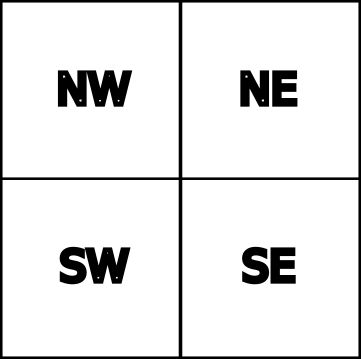
\includegraphics[width=\textwidth]{JudyBenjamin.png}
\caption{Where could Judy Benjamin be?}
\label{f:judybenjamin}
\end{marginfigure}

Initially Judy Benjamin thinks its equally likely she is in any of the quadrants.  Formally she think $P(NW) = P(NE) = P(SW) = P(SE) = \frac{1}{4}$.  Her radio is badly damaged, and just as it is failing she hears an important piece of information from her headquarters:
\begin{quote}
{\it If} you are in the North, we think it's three times more likely that you are in the west.  
\end{quote}
Then the radio fails.

Why this is this a problem? It seems like Judy Benjamin has just learned an important piece of information. She has learned that, whatever her probabilities are it needs to be that $P(NW) = 3 P(NE)$. In fact, it seems quite natural to a lot of people that she should hold fixed $P(SE)$ and $P(SW)$ since she hasn't learned anything about them.  And instead she should adjust $P(NW) = \frac{3}{8}$ and $P(NE) = \frac{1}{8}$.

Unfortunately, Bayes theorem cannot explain our intuitions about this case.  The problem arises because there is no event which corresponds to the radio transmission. Judy Benjamin learned the relationship between two probabilities (or, perhaps, a conditional probability).  But those aren't events.

There are a couple of ways to try and deal with this problem.  One is to adopt other forms of updating that allow for learning arbitrary mathematical constraints. Another is to explicitly expand the set of atomic events so that Judy Benjamin can handle different transmissions from headquarters as events themselves. 

\subsection{Some sentences aren't events}

When I first learned about probability and Bayes theorem, I got really excited about the power to handle uncertainty.  I started thinking about how to apply probability to a large array of different problems.  But, I discovered that it's difficult to always construct the mathematical representation of an event space for every possible sentence.

Take, for example, the sentence ``today is Tuesday.'' This sentence cannot be a simple event in a probability space.  Why not? Well if you assign it probability 1 today, then it had better be probability 0 tomorrow. Then in seven days it will again have probability 1.  Etc.  This cannot be handled by the principle of conditionalization.

There are attempts to expand probability to deal with a broader set of natural language sentences, but it does require work in order to be able to do that.  And of course, the principle of conditionalization will no longer hold in full generality.  Bayes theorem doesn't allow you to go from probability 1 to 0, but that's exactly what I do when I wake up the day after Tuesday.

\section{Conclusion}

There are actually many more potential counter examples to the principle of conditionalization. Philosophers will likely continue to debate it for decades.  I could not hope to give you a full picture of the debate, but here is a taste. If you are interested in learning more, there are many books that go into many more details.

You might have also noted this chapter doesn't have a section on descriptive concerns with the principle of conditionalization.  That in part because it's so difficult to determine if people obey it because, among other things, its difficult to know what people's conditional probabilities are.  Some psychologists think the mind obeys the principle of conditionalization (without us being conscious of it). They think that much about our psychology, like visual illusions and the like, can be explained by our brain updating with Bayes theorem. But there is a debate.

This chapter is a bit of an aside to the rest of the book.  For the remaining chapters, we will return to the comfortable world of the synchronic.  In particular, we will go back to a question we first raised way back in chapter~\ref{c:uncertainty-noprob}, how do we handle uncertainty.  If this book were longer, we could talk about decisions that take place over time, and we could combine this chapter with the next ones.  Alas, it isn't longer (agree with me here\dots please).  So, we won't be able to connect back.